\section{Markt und Preise}
\begin{itemize}
	\item Unbeschränkte Bedürfnisse stehen knappen Ressourcen gegenüber
	\item Wie wird das Budget auf unterschiedliche Verwendungszwecke aufgeteilt
	\item Opportunitätskosten: Kosten, die bei einer Entscheidung anfallen, dass die Vorteile einer Handlungsalternative nicht realisiert werden können
	\item Die Opportunitätskosten zeigen die Knappheit von Gütern in Form von Preisen an
	\item \textbf{Planwirtschaft}
	\subitem Ressourcen gehören Staat
	\subitem Staat lenkt Einsatz
	\item \textbf{Marktwirtschaft}
	\subitem Ressourcen gehören privaten Haushalten und Firmen 
	\subitem Private Haushalte/Firmen entscheiden über Ressourceneinsatz
	\subitem Preis spielt Hauptrolle
\end{itemize}
\subsection{Wirtschaftskreislauf}
\begin{multicols}{2}
	\subsubsection{Einfach}
	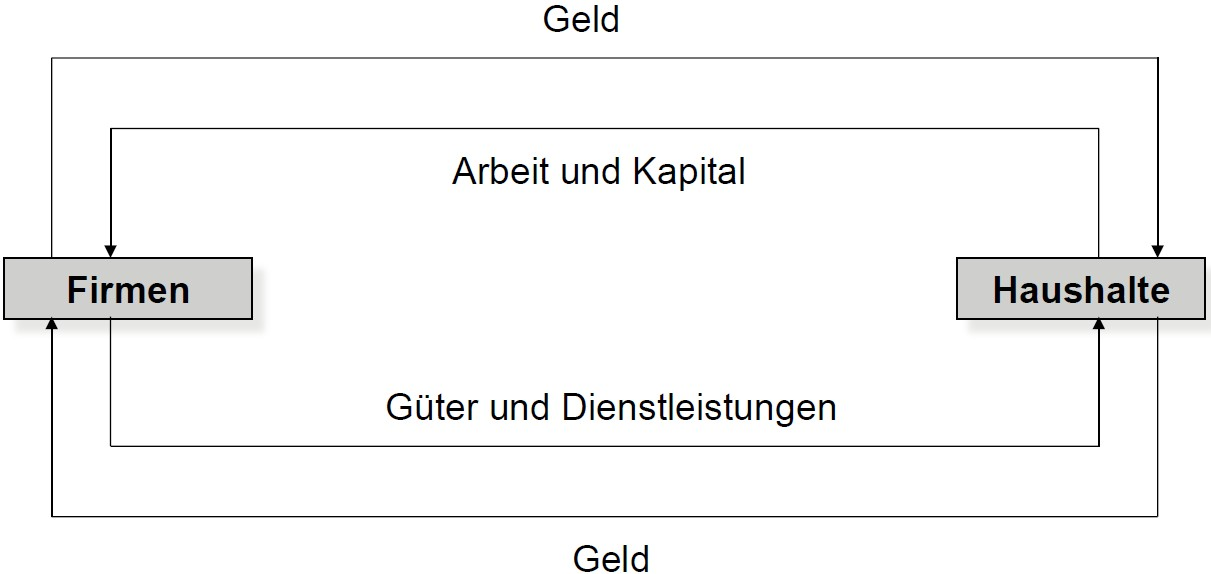
\includegraphics[width=9cm]{images/einfachWS.jpg}
	\subsubsection{Erweitert}
	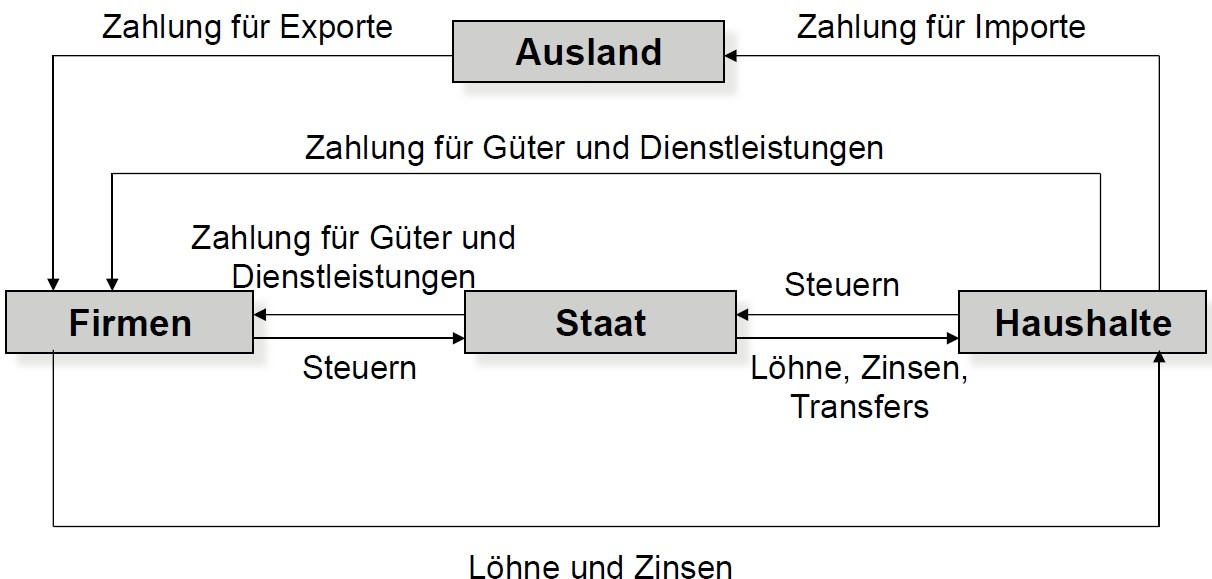
\includegraphics[width=9cm]{images/erweiterWS.jpg}
\end{multicols}
\subsubsection{Märkte}
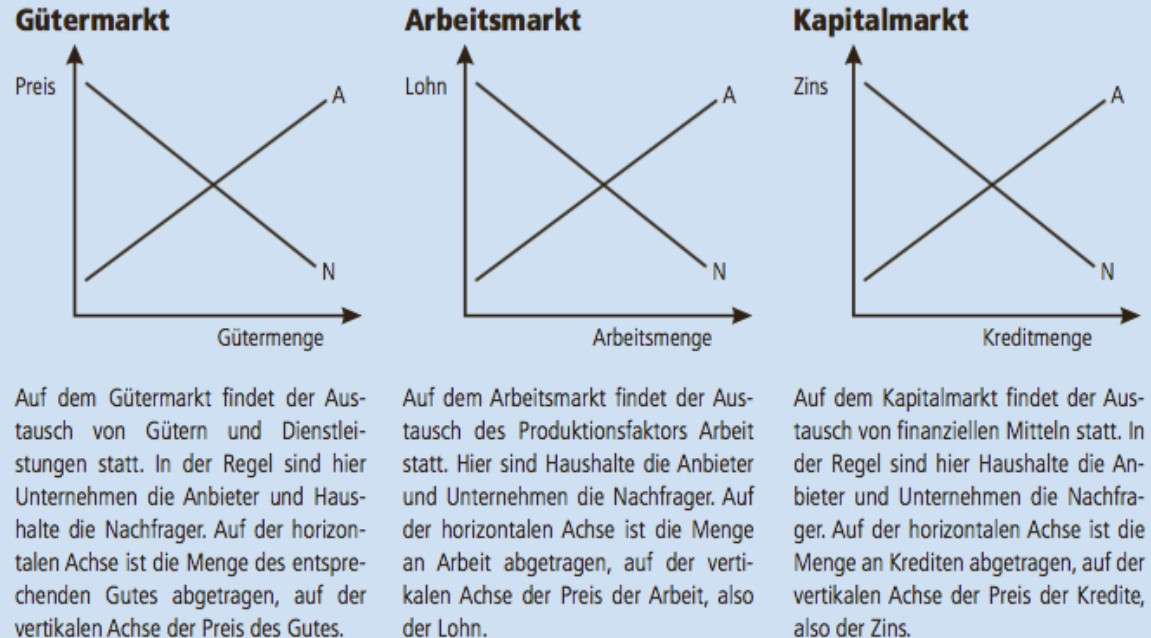
\includegraphics[width=15cm]{images/markte.jpg}
\clearpage
\pagebreak
\subsection{Mikroökonomisches Grundmodell}
\begin{itemize}
	\item Das Gut ist homogen
	\item Es gibt eine grosse Anzahl von Anbietern und Nachfragern
	\item Keine Marktzutrittshemmnisse
	\item Anbieter und Nachfrager sind über Mengen und Preise vollständig informiert
\end{itemize}
\begin{multicols}{2}
	\subsubsection{Konsumentenrente}
	Zahlungsbereitschaft des Käufers für ein Gut,
	abzüglich des Preises, den er tatsächlich dafür bezahlen muss\\
	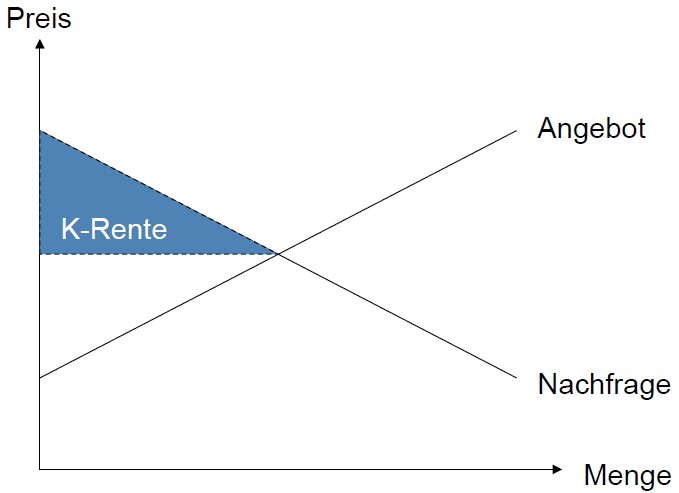
\includegraphics[width=7cm]{images/kr.jpg}
	\subsubsection{Produzentenrente}
	Erlös des Verkäufers für ein Gut, abzüglich der
	Kosten, die ihm für Erwerb oder Herstellung des Gutes entstanden sind\\
	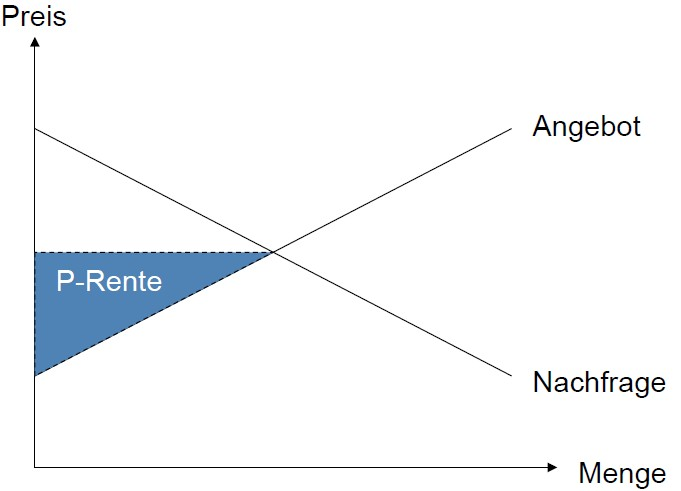
\includegraphics[width=7cm]{images/pr.jpg}
\end{multicols}
\subsubsection{Wohlfahrt}
Gesamte Rente, die auf einem Markt entsteht (Summe
aus Konsumenten- und Produzentenrente)
\begin{figure*}[h]
	\centering
	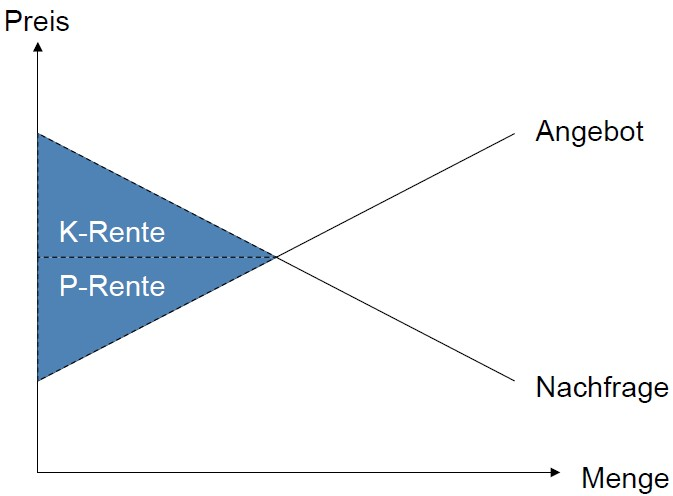
\includegraphics[width=6cm]{images/wohlfahrt.jpg}
\end{figure*}
\subsection{Preiseingriffe}
\begin{multicols}{2}
	\subsubsection{Mindestpreis}
	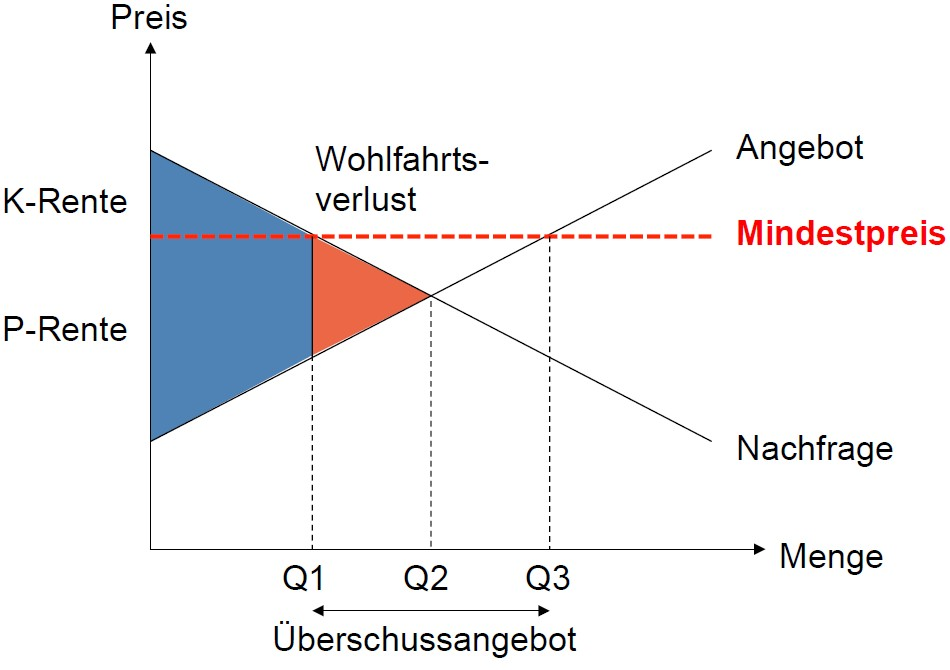
\includegraphics[width=7cm]{images/mindestpreis.jpg}
	\subsubsection{Höchspreis}
	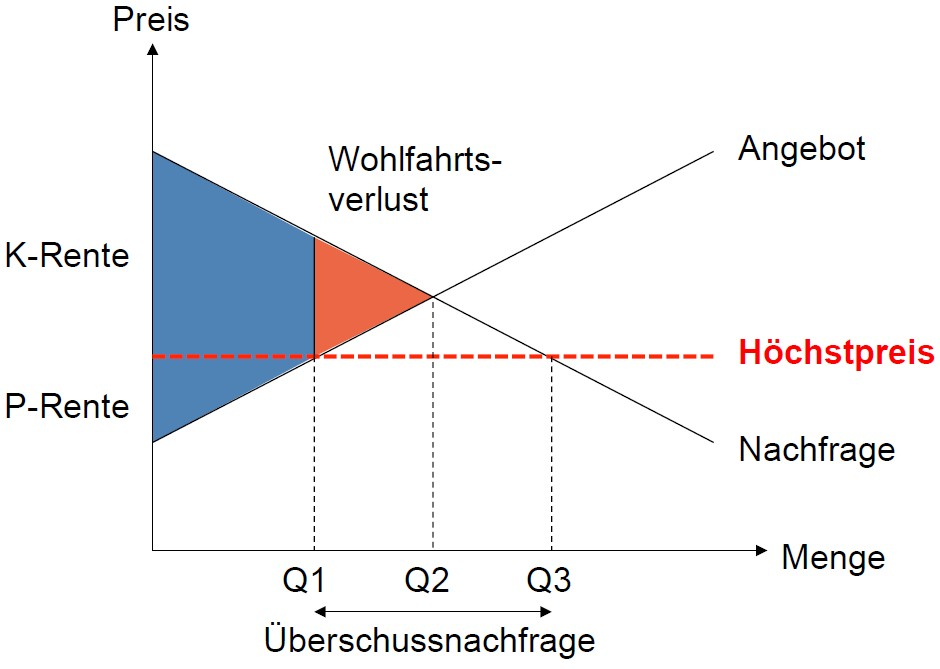
\includegraphics[width=7cm]{images/hochstpreis.jpg}
\end{multicols}

